% XeLaTeX can use any Mac OS X font. See the setromanfont command below.
% Input to XeLaTeX is full Unicode, so Unicode characters can be typed directly into the source.

% The next lines tell TeXShop to typeset with xelatex, and to open and save the source with Unicode encoding.

%!TEX TS-program = xelatex
%!TEX encoding = UTF-8 Unicode





% Will Robertson's fontspec.sty can be used to simplify font choices.
% To experiment, open /Applications/Font Book to examine the fonts provided on Mac OS X,
% and change "Hoefler Text" to any of these choices.



% - Sistemas Operacionais




\hypertarget{sistemas-operacionais}{%
\chapter{Sistemas Operacionais}\label{sistemas-operacionais}}



\hypertarget{Introdução}{%
\section{Introdução}\label{Introdução}}

O Sistema Operacional (SO) é um software que gerencia os recursos de
hardware e os tornam simples de serem usados por aplicações. Esse
gerenciamento é feito pelo núcleo, ou \texttt{Kernel}, do SO, o qual tem
permissões especiais de uso. As aplicações criadas pelos usuários se
encontram no \texttt{User Space}, um local com abstrações para o fácil uso desses
recursos. A mudança do espaço pode ser requisitada pela aplicação, com
um processo chamado de \texttt{trap}, o qual faz referência à uma
interceptação, como cair no alçapão de uma casa, tendo assim acesso ao
subterrâneo, no caso o núcleo do SO. Esse processo passa pelas chamadas
de sistema (System Calls), as quais são uma interface de comunicação
entre o espaço de usuário e o \texttt{kernel}. As aplicações no espaço de usuário
contam com as abstrações GNU libc, uma biblioteca que segue o padrão
POSIX, e outros, de normas de compatibilidade entre os sistemas
operacionais, tornando, assim, os programas portáteis. Outras abstrações
importantes são a de processos, que são programas em execução, e a de
\texttt{File System} (FS), responsável por gerenciar os arquivos, usando, por
exemplo, diretórios para agrupá-los. A inicialização do sistema
computacional começa pelo carregamento do BIOS (\emph{Basic Input Output
System}), o qual é armazenado em uma memória flash (uma EEPROM, ou
\emph{Electrically Erasable and Programmable Read Only Memory}) na placa
mãe, e é encarregado por tarefas básicas de gerenciamento do hardware,
como o POST (\emph{Power On Self Test}), processo incumbido por verificar
o estado operacional do sistema. O BIOS também é responsável por
carregar o SO, da memória secundária para a memória primária, processo
que finaliza com o sistema operacional assumindo o controle do hardware.
A memória primária, ou RAM (\emph{Random Access Memory}), é uma memória
volátil (não mantém os dados após o cessamento da energia) de acesso
direto ao processador. Os programas necessitam estar nessa memória para
serem executados. Já a memória secundária, também chamada de Drive (ou
disco), passa por um sistema I/O (\emph{Input Output}), o qual é
encarregado por gerenciar a entrada e saída de dados com outros
dispositivos. A Figura \ref{fig:sistema computacional} mostra como as subdivisões de um sistema
computacional, destacando as do sistema operacional.

\begin{figure}[h]
\centering
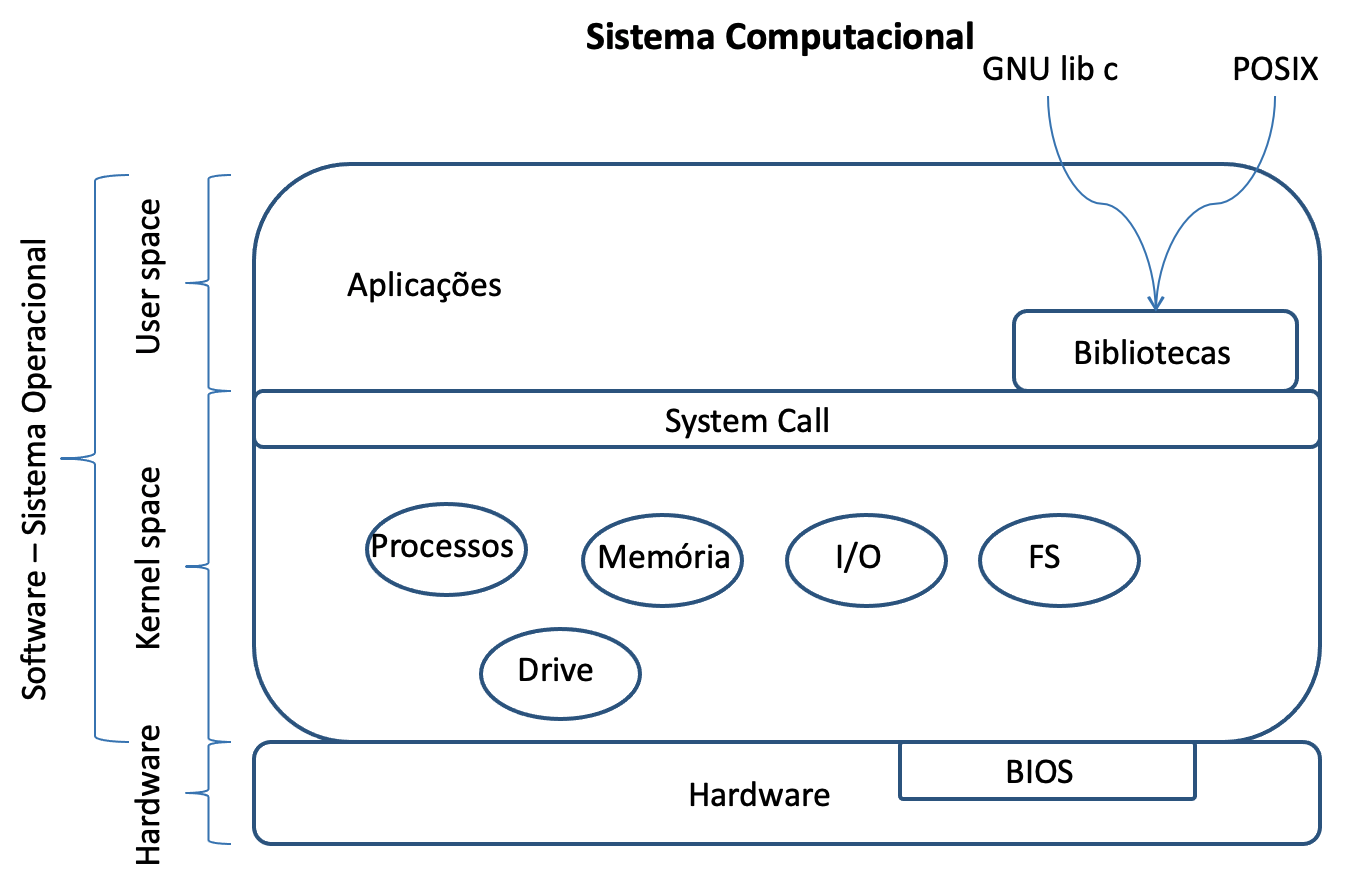
\includegraphics[keepaspectratio, width=12cm, height=9cm]{imagens/02/02 - funcionamento do computador.png}
\caption{Sistema Computacional}
\label{fig:sistema computacional}
\end{figure}



\hypertarget{Prática}{%
\section{Prática}\label{Prática}}

Com o intuito de mostrar como funciona as chamadas do sistema e como
funciona a compilação, vamos criar um programa \texttt{Hello\ world} na
linguagem C. Para tal, precisamos entender alguns comandos do Linux.

\hypertarget{comandos-linux}{%
\subsubsection{Comandos Linux}\label{comandos-linux}}

\begin{enumerate}
\def\labelenumi{\arabic{enumi}.}
\tightlist
\item
  \texttt{mkdir}: cria um novo diretório
\item
  \texttt{grep}: procura um texto em um arquivo
\item
  \texttt{rm}: remover um arquivo
\item
  \texttt{mv}: move o arquivo
\item
  \texttt{ls}: lista os elementos de um diretório
\item
  \texttt{ls\ -a}: lista arquivos
\item
  \texttt{ls\ -l}: lista permissões
\item
  \texttt{ls\ -F}: edita os nomes, como \texttt{*} no final do nome dos
  arquivos executáveis
\item
  \texttt{ls\ -F}: edita os nomes, como \texttt{*} no final do nome dos
  arquivos executáveis
\item
  \texttt{ll}: um alias para \texttt{ls\ -alF}
\item
  \texttt{file}: inspecionar um arquivo
\item
  \texttt{cd}: mudar o diretório
\item
  \texttt{ld}: vinculador, responsável por gerar um arquivo executável a
  partir de um objeto
\item
  \texttt{objdump}: Mostra informações sobre um arquivo objeto
\item
  \texttt{objdump\ -d}: desmota (disassembly) um arquivo objeto.
  
        \begin{lstlisting}[language=bash]
            $ objdump -d file.o
        \end{lstlisting}


\item
  \texttt{Vim}: Vi Improved -- Editor de texto. \texttt{\$vim\ file}
  
        \begin{lstlisting}[language=bash]
            $ vim file
        \end{lstlisting}
\item
  \texttt{Vi}: Editor de texto.
\item
  \texttt{-o}: output -- resultado de um comando
\item
  \texttt{as}: compilador assembly
\item
  \texttt{gcc}: compilador GNU para a linguagem C, gera arquivo
  executável a partir de um arquivo \texttt{.c}.

        \begin{lstlisting}[language=bash]
            $ gcc file.c -o file
        \end{lstlisting}  
  
\item
  \texttt{gcc\ -E}: gera arquivo pré-processado (\texttt{.pre}).
 
  
        \begin{lstlisting}[language=bash]
            $ gcc -E file.c -o file.pre
        \end{lstlisting}  
\item
  \texttt{gcc\ -S}: gera arquivo assembly (\texttt{.s})


        \begin{lstlisting}[language=bash]
            $ gcc -S file.c -o file.s
        \end{lstlisting}  
  
\item
  \texttt{gcc\ -c}: converte em linguagem de máquina sem vincular,
  gerando um arquivo objeto não executável (\texttt{.o})

        \begin{lstlisting}[language=bash]
            $ gcc -c file.c -o file.o
        \end{lstlisting}    
  
\item
  \texttt{man\ \#}: mostra o manual de uma função de alguma sessão


        \begin{lstlisting}[language=bash]
            $ man 3 printf
        \end{lstlisting}      
  
\item
  \texttt{man\ man}: mostra o manual do man
\item
  \texttt{echo}: mostra o texto resultado na saída padrão.
\item
  \texttt{./} : executa um arquivo executável
\end{enumerate}

\hypertarget{etapas-de-compilauxe7uxe3o}{%
\subsection{Etapas de compilação}\label{etapas-de-compilauxe7uxe3o}}

O processo de compilação de um código está relacionado com transformar
um arquivo texto de uma linguagem específica, para um arquivo binário
executável. O compilador da linguagem C usado no Linux, \texttt{gcc},
realiza esse processo em 4 etapas. A primeira dessas etapas é o
pré-processamento, responsável por lidar com as diretivas de
pré-processamento, como o \texttt{\#include} e \texttt{\#define}, que
anexa um arquivo e substitui os macros, respectivamente. Tem como
resultado um arquivo de extensão pre (\texttt{.pre}). A segunda etapa é
a conversão do arquivo pré-processado para o assembly. Ela utiliza o
\emph{toolchain}, pacote de ferramentas contendo instruções específicas
do processador de destino, como ARM. A saída é um arquivo de extensão s
(\texttt{.s}). A terceira etapa é a geração de um código objeto em
binário, o qual é um arquivo de extensão o (\texttt{.o}). Por fim, há a
vinculação (\emph{linking}) do código objeto gerado na etapa anterior
com outros códigos objetos a fim de substituir as referências à símbolos
definidos fora do código objeto original. Tem como saída um arquivo
binário executável sem extensão. A Figura \ref{fig:Etapas de compilação do gcc} mostra as etapas de
compilação do gcc.

\begin{figure}[h!]
\centering
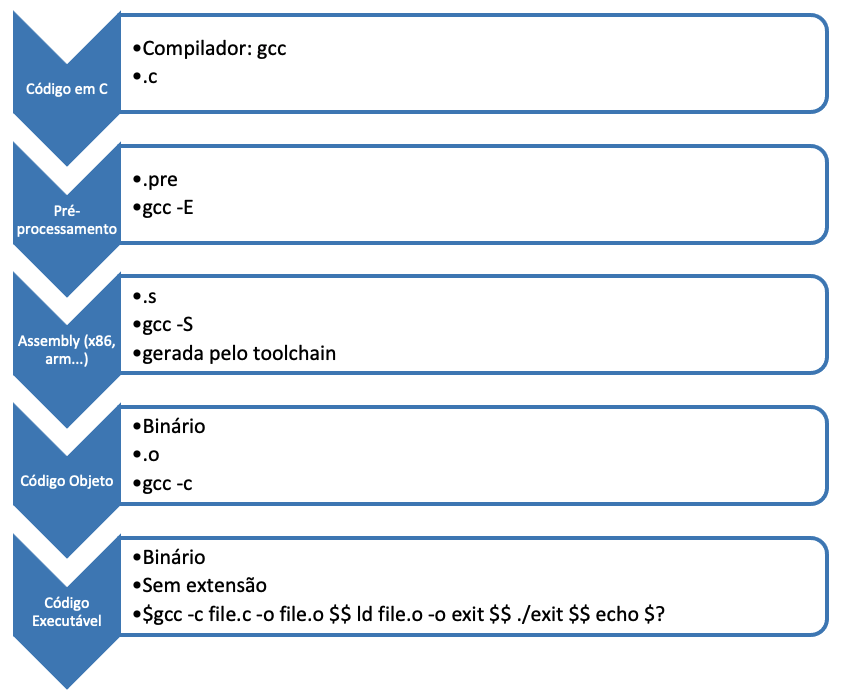
\includegraphics[width=12cm, height=9cm]{imagens/02/02 - compilação.png}
\caption{Etapas de compilação do gcc}
\label{fig:Etapas de compilação do gcc}
\end{figure}




\hypertarget{compilando-um-arquivo-.c}{%
\section{\texorpdfstring{Compilando um arquivo
\texttt{.c}}{Compilando um arquivo .c}}\label{compilando-um-arquivo-.c}}

A seguir será mostrado um passo a passo, da criação de um arquivo
\texttt{.c} até sua compilação.

Dentro do editor de texto Linux, escreva o código \texttt{Hello\ World}
disponível a seguir.

\begin{minted}[mathescape, linenos]{c}

    #include <stdio.h>
    int main() { 
        printf("Hello World!\n); 
        return 0; 
    }

\end{minted}



Salve com o nome \texttt{hw.c} Abra o terminal, vá até o diretório no
qual foi salvo o arquivo \texttt{hw.c}, e digite:


\begin{lstlisting}[language=bash]
  $ gcc hw.c -o hw
  $ ./hw
\end{lstlisting}





Será assim gerado um arquivo \texttt{hw} executável, com sua execução em
seguida.

Com o \texttt{gcc}, pode-se também gerar os arquivos das etapas
explicadas anteriormente, com 1, 2 e 3 gerando os arquivos
pré-processados, arquivo assembly e código objeto, respectivamente.





\begin{minted}[mathescape, linenos]{bash}

    $ gcc -E hw.c -o hw.pre
    $ gcc -S hw.c -o hw.s
    $ gcc -c hw.c -o hw.o
\end{minted}



É possível também ler o código objeto no formato de assembly com a
função de desassembly:

\begin{minted}[mathescape, linenos]{language=bash}

    $ objdump -d hw.o
    
    hw.o:     file format elf64-x86-64
    
    
    Disassembly of section .text:
    
    0000000000000000 <main>:
       0:   f3 0f 1e fa             endbr64
       4:   55                      push        %rbp
       5:   48 89 e5                mov         %rsp,%rbp
       8:   48 8d 3d 00 00 00 00    lea         0x0(%rip),%rdi  # f <main+0xf>
       f:   b8 00 00 00 00          mov         $0x0,%eax
      14:   e8 00 00 00 00          callq       19 <main+0x19>
      19:   b8 00 00 00 00          mov         $0x0,%eax
      1e:   5d                      pop         %rbp
      1f:   c3                      retq
\end{minted}


\hypertarget{executando-uma-chamada-do-sistema}{%
\section{Executando uma chamada do
sistema}\label{executando-uma-chamada-do-sistema}}

Para executar uma chamada do sistema, vamos, primeiro, criar um arquivo
assembly (\texttt{.s}) chamado de \texttt{01-exit64.s} com o conteúdo
abaixo:

\begin{minted}[mathescape, linenos]{assembly}
    
    .section .data
    .section .text
    .globl _start
    
    _start:
    
    
    # C code
    # exit(0);
        # mnemonic  # parameters    # comments
        movq        $60, %rax   # system call exit(2)
        movq        $10, %rdi   # the shell will receive this value
    
        syscall
\end{minted}



Após isso, devemos gerar um código objeto, usando um compilador assembly:

\begin{lstlisting}[language=bash]
    $ as 01-exit64.s -o exit.o
\end{lstlisting}



Depois gerar um arquivo executável, pelo processo de vinculação:


\begin{lstlisting}[language=bash]
    $ ld exit.o -o exit
\end{lstlisting}


Para executar e visualizar, basta digitar:


\begin{lstlisting}[language=bash]
    $ ./exit
    $ echo $?
\end{lstlisting}



\hypertarget{entendendo-system-call}{%
\subsection{Entendendo System Call}\label{entendendo-system-call}}

Para entender melhor o resultado gerado anteriormente, podemos acessar o
manual do system call com:


\begin{lstlisting}[language=bash]
    $ man syscall
\end{lstlisting}



A primeira tabela do manual será parecida com a tabela a seguir:




\begin{table}[h!]
\centering
\begin{tabular}{||c c c c c c||} 
 \hline
    Arch / ABI & Instruction & System Call # & val & val 2 & Error \\ [0.5ex] 
 \hline\hline
arm64 & svc \#0 & x8 & 0 & x1 & - \\
 \hline
 i386 & int \$0x80 & eax & ax & edx & - \\
 \hline
 mips & syscall & v0 & 0 & v1 & a3 \\
 \hline
 riscv & ecall & a7 & 0 & a1 & - \\
 \hline
 x86-64 & syscall & rax & ax & rdx & - \\
 \hline
 x32 & syscall & a2 & 2 & - & - \\
 \hline

\end{tabular}


 \caption{System Call por Arquitetura}
\label{tab:System Call por Arquitetura}
\end{table}


A Tabela \ref{tab:System Call por Arquitetura} mostra que para que a função syscall de um processador com
arquitetura x86-64 seja chamada, devemos primeiro ajustar o registrador
rax com o valor equivalente à função desejada. No exemplo dado, o valor
60 se refere a função ``exit'', que encerra a execução de um programa.
As diferentes funções e seus respectivos valores podem ser acessados em:

\url{https://elixir.bootlin.com/linux/latest/source/arch/x86/entry/syscalls/syscall\_64.tbl}

A Tabela \ref{tab:Argumentos das chamadas do sistema} mostra que o primeiro argumento a ser usado na arquitetura
x86-64 deve ser passado para o registrador rdi. A tabela completa pode
ser encontrada no manual do syscall. O valor passado para esse
registrador será retornado pelo syscall.



\begin{table}[h!]
\centering
\begin{tabular}{||c c c c c c c c c||} 
 \hline
    Arch / ABI & rg1 & rg2 & rg3 & rg4 & rg5 & rg6 & rg7 & notes \\ [0.5ex] 
 \hline\hline
x86-64 & rdi & rsi & rdx & r10 & r8 & r9 & - & \\

 \hline

\end{tabular}

 \caption{Argumentos das chamadas do sistema}
\label{tab:Argumentos das chamadas do sistema}
\end{table}

\somestuffstyle{movq}
A função \texttt{movq}, utilizada no programa assembly, move o valor
especificado para um dado registrador. No exemplo, movemos o valor 60
para o registrador \texttt{rax}, e o valor 10 para o registrador
\texttt{rdi}. A instrução syscall, que, como mostrado na Tabela 1, usa o
valor contido no registrador \texttt{rax}, no caso 60, para fazer
referência a função a ser chamada, e, como argumento, é passado o valor
10 para o registrador \texttt{rdi} que, como pode ser visto na Tabela 2,
se refere ao primeiro argumento de uma syscall. Ao ser executada, a
instrução syscall bloqueia o programa e passa o controle ao sistema
operacional, para que assim possa processar a função requisitada no
kernel space, retornando, no final da execução, ao programa. No caso, o
syscall terá como retorno o próprio argumento, o valor 10, que é visto
usando a função \texttt{echo\ \$?}. É interessante notar que, ao usar a
função \texttt{objdump\ -d} com o arquivo \texttt{exit.o}, é possível
ver que os números 60 e 10 foram substituídos por 0x3c e 0xa. O valor 0x
é uma referência para hexadecimal, e os valores ``3c'' e ``a'' são os
equivalentes a 60 e 10 em hexadecimal.